%%%%%%%%%%%%%%%%%%%%%%%%%%%%%%%%%%%%%%%%%%%%%%%%%%%%%%%%%%%%%%%%%%%%%%%%%%%
%% This file is part of the book
%%
%% Algorithmic Graph Theory
%% http://code.google.com/p/graph-theory-algorithms-book/
%%
%% Copyright (C) 2009--2011 Minh Van Nguyen <nguyenminh2@gmail.com>
%%
%% See the file COPYING for copying conditions.
%%%%%%%%%%%%%%%%%%%%%%%%%%%%%%%%%%%%%%%%%%%%%%%%%%%%%%%%%%%%%%%%%%%%%%%%%%%

\documentclass{article}

\usepackage{tikz}
\usetikzlibrary{external}
\tikzexternalize{random-oriented-graph}

\begin{document}

\begin{figure}
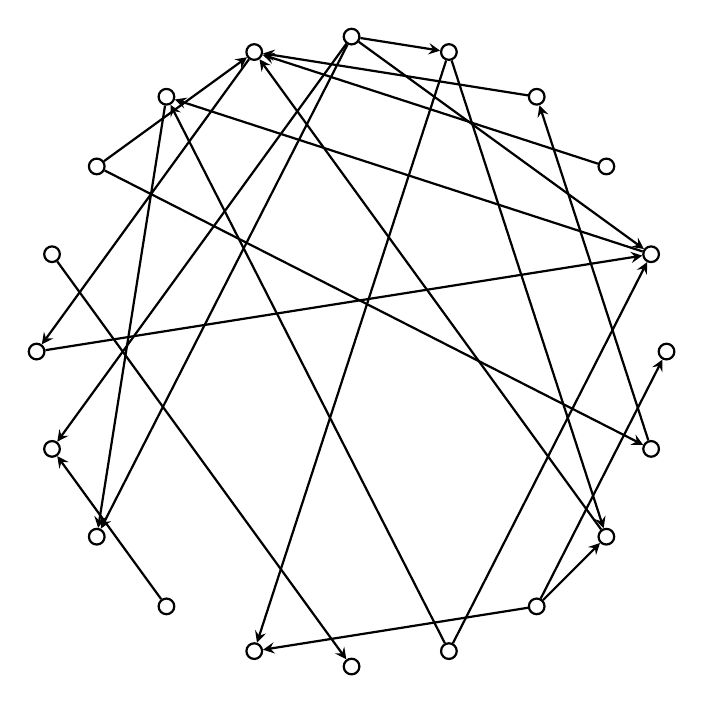
\begin{tikzpicture}
[lineDecorate/.style={->,>=stealth,thick},%
  nodeDecorate/.style={shape=circle,inner sep=2pt,draw,thick},
  scale=4]
%% nodes or vertices
\foreach \nodename/\x/\y in {
  0/1.00000000000000/0.000000000000000,
  1/0.951056516295154/0.309016994374947,
  2/0.809016994374947/0.587785252292473,
  3/0.587785252292473/0.809016994374947,
  4/0.309016994374947/0.951056516295154,
  5/0.000000000000000/1.00000000000000,
  6/-0.309016994374947/0.951056516295154,
  7/-0.587785252292473/0.809016994374947,
  8/-0.809016994374947/0.587785252292473,
  9/-0.951056516295154/0.309016994374947,
  10/-1.00000000000000/0.000000000000000,
  11/-0.951056516295154/-0.309016994374947,
  12/-0.809016994374947/-0.587785252292473,
  13/-0.587785252292473/-0.809016994374947,
  14/-0.309016994374947/-0.951056516295154,
  15/0.000000000000000/-1.00000000000000,
  16/0.309016994374947/-0.951056516295154,
  17/0.587785252292473/-0.809016994374947,
  18/0.809016994374947/-0.587785252292473,
  19/0.951056516295154/-0.309016994374947}
{
  \node (\nodename) at (\x,\y) [nodeDecorate] {};
}
%% edges or lines
\path
\foreach \startnode/\endnode in {
  1/7, 2/6, 3/6, 4/14, 4/18, 5/1, 5/4, 5/11, 5/12, 6/10, 7/12, 8/6,
  8/19, 9/15, 10/1, 13/11, 16/1, 16/7, 17/0, 17/14, 17/18, 18/6, 19/3}
{
  (\startnode) edge[lineDecorate] node {} (\endnode)
};
\end{tikzpicture}
\end{figure}

\end{document}
